\chapter{Background}
\doublespacing
\label{chap:background}
\minitoc


\section{Introduction}
In this chapter, we review the related topics for the background knowledge for this thesis and provide a state of the art review of related literature. First, We summerize background knowledge on social Web and semantic Web.
Second, we provide an introduction to the collaborative project OCKTOPUS in which this Ph.D. took place.
We then discuss the state of the art approaches to community detection, topic modelling and temporal analysis in question-answering sites, and to question-answering site management. 
Finally, we define the focus of this thesis by identifying the research questions addressed and by  positioning our contribution with regard to the state of the art.

\section{Social Semantic Web: combine social network analysis and Semantic Web}

\subsection{Social Web: online communities and user-generated content}
The term "social Web" was coined by Howard Rheingold in 1996. His Whole Earth Review article in 1987 introduced the notion of “Virtual Communities” and he was quoted in an article in Time magazine in 1996 introducing the term "Social Web". His website "Electric Minds", described as a "virtual community", listed online communities for users interested in socializing through the Web, stating that "the idea is that we will lead the transformation of the Web into a social Web" \cite{rheingold2000virtual}. According to the World Wide Web Consortium (W3C), "the Social Web is a set of relationships that link together people over the Web"\footnote{\url{https://www.w3.org/2005/Incubator/socialweb/XGR-socialweb-20101206/}(accessed Feb 2016)}. The social Web is designed and developed to support social interaction  \cite{porter2010designing} on the Web. These on-line social interactions include for instance online shopping, blogs, forums, video sharing and social networking websites. Today, hundreds of millions of persons are using thousands of social websites to connect with friends, discover news and to share user-generated content, such as blogs, photos, microblogs, videos. By the end quarter of 2008, Facebook reported 67 million members, YouTube had more than 100 million videos and 2.9 million user channels  \cite{watson2008causewired}, and these numbers are consistently growing, as today Facebook reports more than a billion of active users.  


\subsubsection{Web 2.0}
One of the significant changes for the World Wide Web was to move from the parctices of Web 1.0 to the practices of Web 2.0. The term Web 2.0 was initially coined by Darcy DiNucci in 1999  \cite{dinucci2012fragmented} and became popular through Tim O'Reilly in 2005 \cite{o2009design}. Web 2.0 techniques allowed Users to interact and collaborate with each other and create user-generated content in online community sites, while users were mostly browsing content on Web 1.0 sites. A comparison of examples of traditional Web 1.0 sites and Web 2.0 sites is hown in Figure \ref{fig:web1to2}. Popular examples of Web 2.0 sites are Facebook (social networking service), Twitter (a microblog), Youtube (a video-sharing website), Reddit (a user-generated news website).

\begin{figure}%[htbp]
\centering
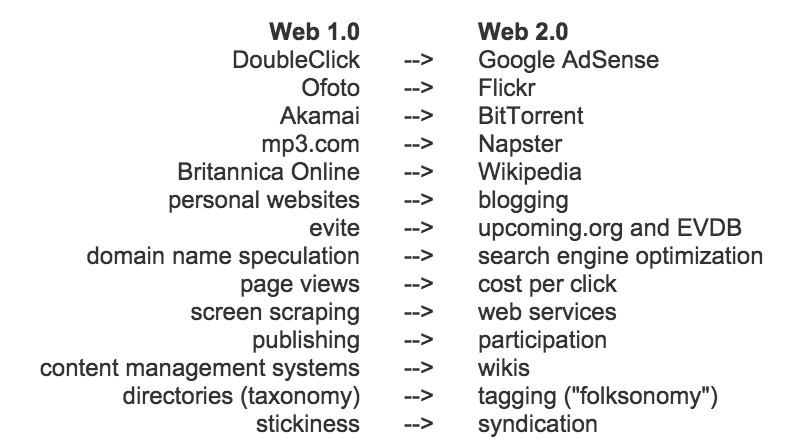
\includegraphics[width=3.2in]{web1to2.jpeg}  
\caption{A comparison of examples of Web 1.0 and Web 2.0 sites, as in \cite{o2009design}}
\label{fig:web1to2} 
\end{figure}
With the evolution of web development technologies, such as Asynchronous JavaScript and XML (AJAX), Rich Internet Applications(RIA), Cascading Style Sheets (CSS), etc. Web 2.0 allowed users to create and share richly-typed user-generated content more easily. \cite{passant2009technologies} argue that there are two main principles in Web 2.0, the first one is the \textit{"Web as a platform"}, which implies the migration from traditional desktop applications (email clients, office suites, etc.) to Web-based applications. The second one is the \textit{"architecture of participation"}, which represents how users change from data consumers to data producers in Web-based applications. For a more detailed description of the design principles of Web 2.0 websites, we refer the reader to \cite{o2009design}. 


\subsubsection{User-generated content}
The OECD~\cite{web2007web} considers that User-Generated Content (UGC) applications have the following requirements: 1) a content which is made publicly available through Internet, 2) boasting a certain level of creativity and, maybe the most important point, 3) contents created outside of professional practices. UGC can be any form of content such as blog posts, photos, questions and answers, forums, tweets, videos, etc., created by users of online social media websites. \cite{moens2014mining} The reasons why people contribute to user-generated content are many: connecting with people, self-expression and receiving recognition. For example: users connect with friends on Facebook; users express themselves on Twitter\footnote{\url{https://twitter.com/}(accessed Feb 2016)}; users share their photos on Flickr\footnote{\url{https://www.flickr.com/} (accessed Feb 2016)}; Users ask and answer computer programming related questions on StackOverflow\footnote{\url{http://stackoverflow.com/} (accessed Feb 2016)}. 

Nevertheless, there are some issues \cite{balasubramaniam2009user} about UGC, such as: the trust problem, since the content is written by non-professionals; the privacy problem, since the content often contains or reveals private information; the copyright problem, more attention should be put on protecting the rights on user-generated content; etc.
For more detailed information about the driving factors and the evolution of UGC, the commercial influence of UGC, we refer the readers to \cite{balasubramaniam2009user} and \cite{smith2012does}.

\subsubsection{Question-and-Answer (Q\&A) sites}

Question-and-Answer (Q\&A) sites, also refered to as Community Question Answering (CQA) sites, initially aimed at enabling users to ask questions to a community of experts or, at least, a community of (shared) interest. Since this user-generated content, composed of questions and answers in this case, can be archived and later viewed and searched again, people with the same or similar questions can find answers by browsing or searching the questions that were already answered. For example\footnote{\url{https://en.wikipedia.org/wiki/Comparison_of_Q\&A_sites} (accessed Feb 2016)},
%TODO FAB : Naver does not appear in Wikipedia comparison
%DONE, it's naver knowledge serach
the first potential Q\&A site Naver Knowledge Search \footnote{\url{http://naver.com} (accessed Feb 2016)} launched in 2002 in Korean, has accumulated 70 million questions and answers, and continues to receive over 40,000 questions and 110,000 answers per day~\cite{sanghunnewyork}. Baidu Knows\footnote{\url{http://zhidao.baidu.com/} (accessed Feb 2016)} and Zhihu \footnote{\url{http://www.zhihu.com/} (accessed Feb 2016)} are the most popular Q\&A sites in China. It is reported \footnote{\url{https://en.wikipedia.org/wiki/Zhihu} (accessed Feb 2016)} that the number of registered users of Zhihu had exceeded 10 millions at the end of 2013, and reached 17 millions in May 2015 with 250 million page views monthly. Yahoo Answers, launched in 2005, offers Q\&A sites localized in 26 countries and according to~\cite{Harper:2008:PAQ:1357054.1357191} in September 2007 it was estimated having 18 millions unique visitors monthly.


As the main access means to information on the Web are the search engines, we compare the traditional keyword-based search engine to Q\&A sites in terms of information retrieval tasks. In search engines, people choose some keywords to describe their problem, then look for related information in the result pages to solve their problems. In Q\&A sites, people post their questions and wait for experts to solve it. Table \ref{tab:intro_compare} compares the two paradigms. 
\begin{table}[!hbp]
\tiny
\centering
\begin{tabular}{|p{50pt}|p{60pt}|p{60pt}|p{60pt}|p{60pt}|}
%\begin{tabular}{|c|c|c|c|c|}
\hline
& Problem definition & Answer time & Results Precision & Problem Answers \\
\hline
Q\&A & Well organized questions and background information & Until someone answers it & Specific to the question& Directly get the answers\\
\hline
Search Engine& Well chosen keywords or short question & Immediately get relevant information & Not specific to the question& Need to analyze the results\\
\hline
\end{tabular}
\caption{Comparison of Q\&A sites and Search Engines}
\label{tab:intro_compare}
\end{table}

In a Q\&A site, people need to provide very detailed information about their questions, in order to let other users understand them. Providing additional details is even often asked by the experts in the first interactions. In a search engine, people have to wisely choose search keywords in order to look for solutions as the quality of keywords largely influences the results. When we pose a question to a Q\&A site, it takes time to attract expert users and get the answers, but the search engine can immediately return relevant information. Once people get an answers from Q\&A site, normally it is very specific to the question and very precise. So Q\&A site can solve very complicated and precise questions. In search engine, people can get very relevant information about the keywords they provide but sometime, the results are very general and not specific to the question. User then have to find the solutions from the provided information by themselves. Beyond this comparison, it must also be stressed that as a Q\&A site grows, priding an efficient search engine for its archive becomes a specific problem at the intersection of both paradigms. Moreover, a number of results found by major search engines come from Q\&A Web archives.

On one hand, Q\&A sites became huge repositories of question-answer content which provide highly valuable and highly reusable knowledge \cite{anderson2012discovering}, \cite{Shah:2010:EPA:1835449.1835518}. On the other hand, Q\&A sites also contain a large number of users who keep contributing questions and answers. And most of them are more likely to ask questions on topics they are interested in and answer questions in topics they are experts of. This strong coupling of linked content and linked users is an aspect we will come back to.

Thus, we can consider this user-generated content is normally of high quality as it was generated by people with very strong domain knowledge and expertise. We list key features of some famous Q\&A sites in table \ref{tab:qasites}. 
The column 'Category' indicates the topics which are discussed in the websites.
The column 'Reward' indicates the rewarding system which is used to encourage users' contribution.
The column 'Tag' indicates whether the website enables users to assign tags on questions.
The column 'Vote' indicates whether the website enables users to vote on questions, answers or both.
The column 'Best Answer' indicates whether the website enables users to choose a best answer.



\begin{sidewaystable}%[!hbp]
\centering
%\begin{tabular}{|p{46pt}|p{60pt}|p{60pt}|p{25pt}|p{60pt}|p{25pt}|}
\begin{tabular}{|c|c|c|c|c|c|c|}
\hline
& Category & Reward &  Tag & Vote & Best Answer & Dataset availability\\
\hline
Yahoo Answer\footnote{\url{https://answers.yahoo.com/} (accessed Feb 2016)} & Multiple & Level and Points & no& answer & yes & Web access\\
\hline
StackOverflow\footnote{\url{http://stackoverflow.com/} (accessed Feb 2016)} & Computer Science & Reputations & yes & both & yes& full access\footnote{\url{https://archive.org/details/stackexchange} (accessed Feb 2016)} \\
\hline
Baidu Zhidao\footnote{\url{http://zhidao.baidu.com/} (accessed Feb 2016)}& Multiple&Level and Coins & no &both & yes& Web access \\
\hline
Zhihu\footnote{\url{https://www.zhihu.com/} (accessed Feb 2016)} & Multiple & Vote and Like & yes & answer & yes& Web access \\
\hline
Quora\footnote{\url{https://www.quora.com/} (accessed Feb 2016)} & Multiple&views& no & answer & no & Web access\\
\hline
\end{tabular}
\caption{Key features of famous Q\&A sites}
\label{tab:qasites}
\end{sidewaystable}

StackOverflow is the most popular Q\&A site that focus on computer programming topics. Its data is published every month. It includes all the detailed information, such as quesiton answer contents, user profile, temporal information. This is why we decided to use StackOverflow dataset throughout this work. Figure \ref{fig:stackexample} shows an example of question and answer on StackOverflow.  
\begin{figure}%[htbp]
\centering
%\epsfig{file=fly.eps, height=1in, width=1in} % use this if you use "pdflatex"
%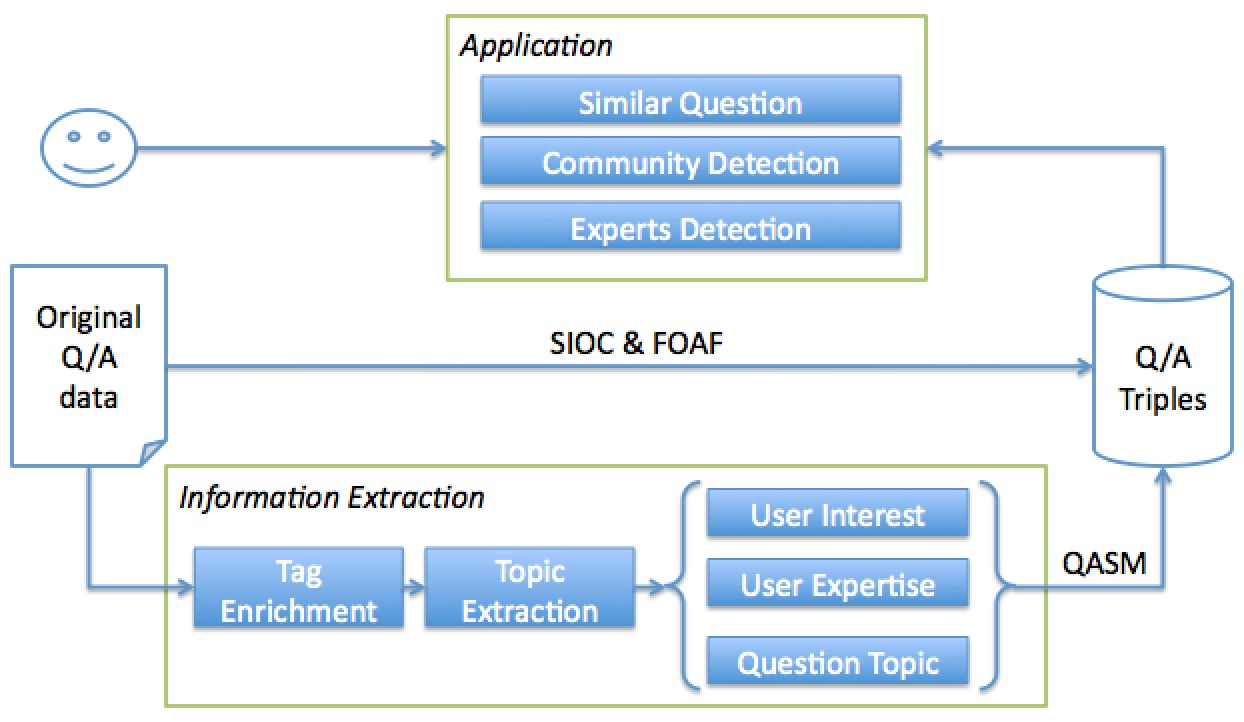
\includegraphics[height=1.857in, width=3.2in]{overview.png}  
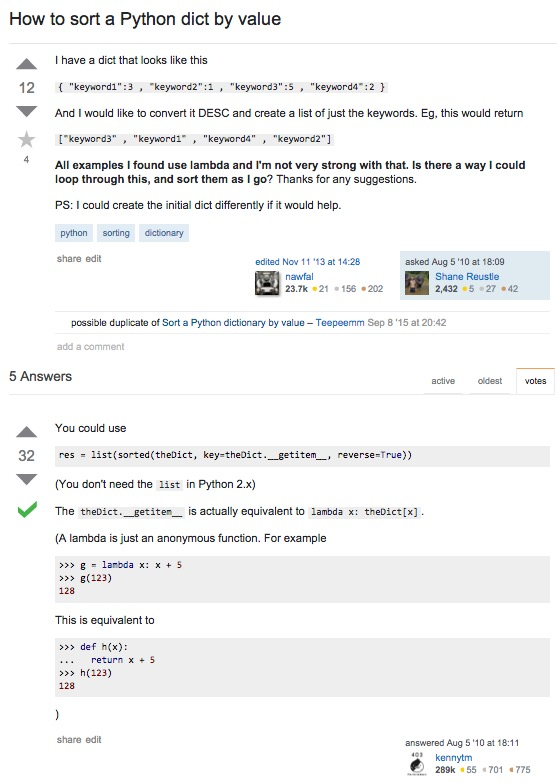
\includegraphics[width=5.3in]{stackexample.jpeg}  
\caption{A example of question and answer on StackOverflow \footnote{\url{http://stackoverflow.com/questions/3417760/how-to-sort-a-python-dict-by-value} (accessed Feb 2016)}}
\label{fig:stackexample} 
\end{figure}

As already pointed, there are two main dimensions in Q\&A sites, the coupling of which provide the power of these sites:
\begin{itemize}
\item{Social dimension:} 
A large number of people are very active and keep contributing answers to these sites. Most of them are more likely to answer questions about topics in which they are interested and specialized. Identifying interest groups of users in Q\&A sites is an interesting indication of expertize in a Q\&A and community detection is a fundamental research topic for social network analysis. Many community detection algorithms have been developed to find sub-structures in social networks. Q\&A sites are also social networks. However, unlike friendship networks such as Facebook, there are no explicit relationships between people on Q\&A sites. Besides people are not aware of who they are interacting with, and normally they do not maintain a solid relationship. People are more like isolated nodes grouped by interests and the social network remains implicit. So interest groups are an important implicit sub-structure to detect in such social sites. Moreover, people have multiple interests and therefore belong to several interest groups. Therefore an important aspect is the ability to detect overlapping communities or interest. 

\item{Content dimension:}
Another important resource in Q\&A sites are "question-answer" pairs. Questions cover different topics, and the fact that a user asks or answers a question can reflect the fact that he/she is interested in the topics touched by that question. Therefore, detecting topics of questions and identifying interests of groups are related problems. We want not only to detect communities, but also to find their "raison d'\^etre" i.e. to find the topic(s) of interest shared by each detected community. Topic extraction is a critical research problem in text analysis. Many topic extraction methods have been proposed to cluster textual resources by their topics. One of the reasons why we need such content analysis is that it enables systems, for instance, to use topics in recommending similar questions or in routing questions to experts, which are both very important functionalities in Q\&A scenarios.

\end{itemize}

\subsection{Semantic Web: formalizing and linking knowledge}

According to the W3C, "The Semantic Web provides a common framework that allows data to be shared and reused across application, enterprise, and community boundaries"\footnote{\url{https://www.w3.org/2001/sw/} (accessed Feb 2016)} through the Web. Tim Berners-Lee \cite{berners2001semantic} also uses this term to refer to a Web of data that can be processed by machines. It is a change from a vision of a Web of documents to a Web also publishing and linking datasets. People generate and consume huge amounts of data every day. However, these data are kept in silos by each application or each website, and people have to manage and process the exchange of information by themselves. For example, in order to make a trip plan, a user should check different websites including flight, hotel, weather, train schedule and so on. It is even not easy for a human to integrate them. For example, a small change of flight may cause the user to check and change all the other reservations. It is also not possible for applications to manage all these information from different websites. However, with a Web of data instead of a Web of document, it becomes possible for applications to process and integrate data together. So, a key attribute of the Semantic Web is to enable content providers not only to publish human-readable Web documents, but also machine-readable data. With this vision, the Semantic Web allows applications to process data from different sources the same way people gather information from different Web pages. 
Later in 2006, Tim Berners-Lee\cite{berners2006linked} proposed the Linked Data principles for publishing structured data on the Semantic Web. It is a method to share Semantic Web data using the Web architecture \cite{bizer2011evolving}. An important development in this context is the W3C Linking Open Data (LOD) \footnote{\url{https://www.w3.org/wiki/SweoIG/TaskForces/CommunityProjects/LinkingOpenData} (accessed Feb 2016)}. Figure \ref{fig:lod} shows the LOD cloud diagram\footnote{Linking Open Data cloud diagram, by Richard Cyganiak and Anja Jentzsch. \url{http://lod-cloud.net/}}. It shows the datasets that have been published as Linked Data. As of August 2014, the LOD cloud contains 1014 data sets classified into 8 domains while there are 520 datasets (taking 51.28\%) in the domain of Social Web and 48 datasets in User-generated contents (taking 4.73\%).


In the following subsections, we briefly introduce the RDF data model which is used to represent data on the Semantic Web and the related vocabularies to formalize social media datasets. For more details about the objectives and goals of the Semantic Web, we refer the readers to \cite{feigenbaum2007semantic} and \cite{berners2001semantic}.

\begin{sidewaysfigure}%[htbp]
\centering
%\begin{sideways}
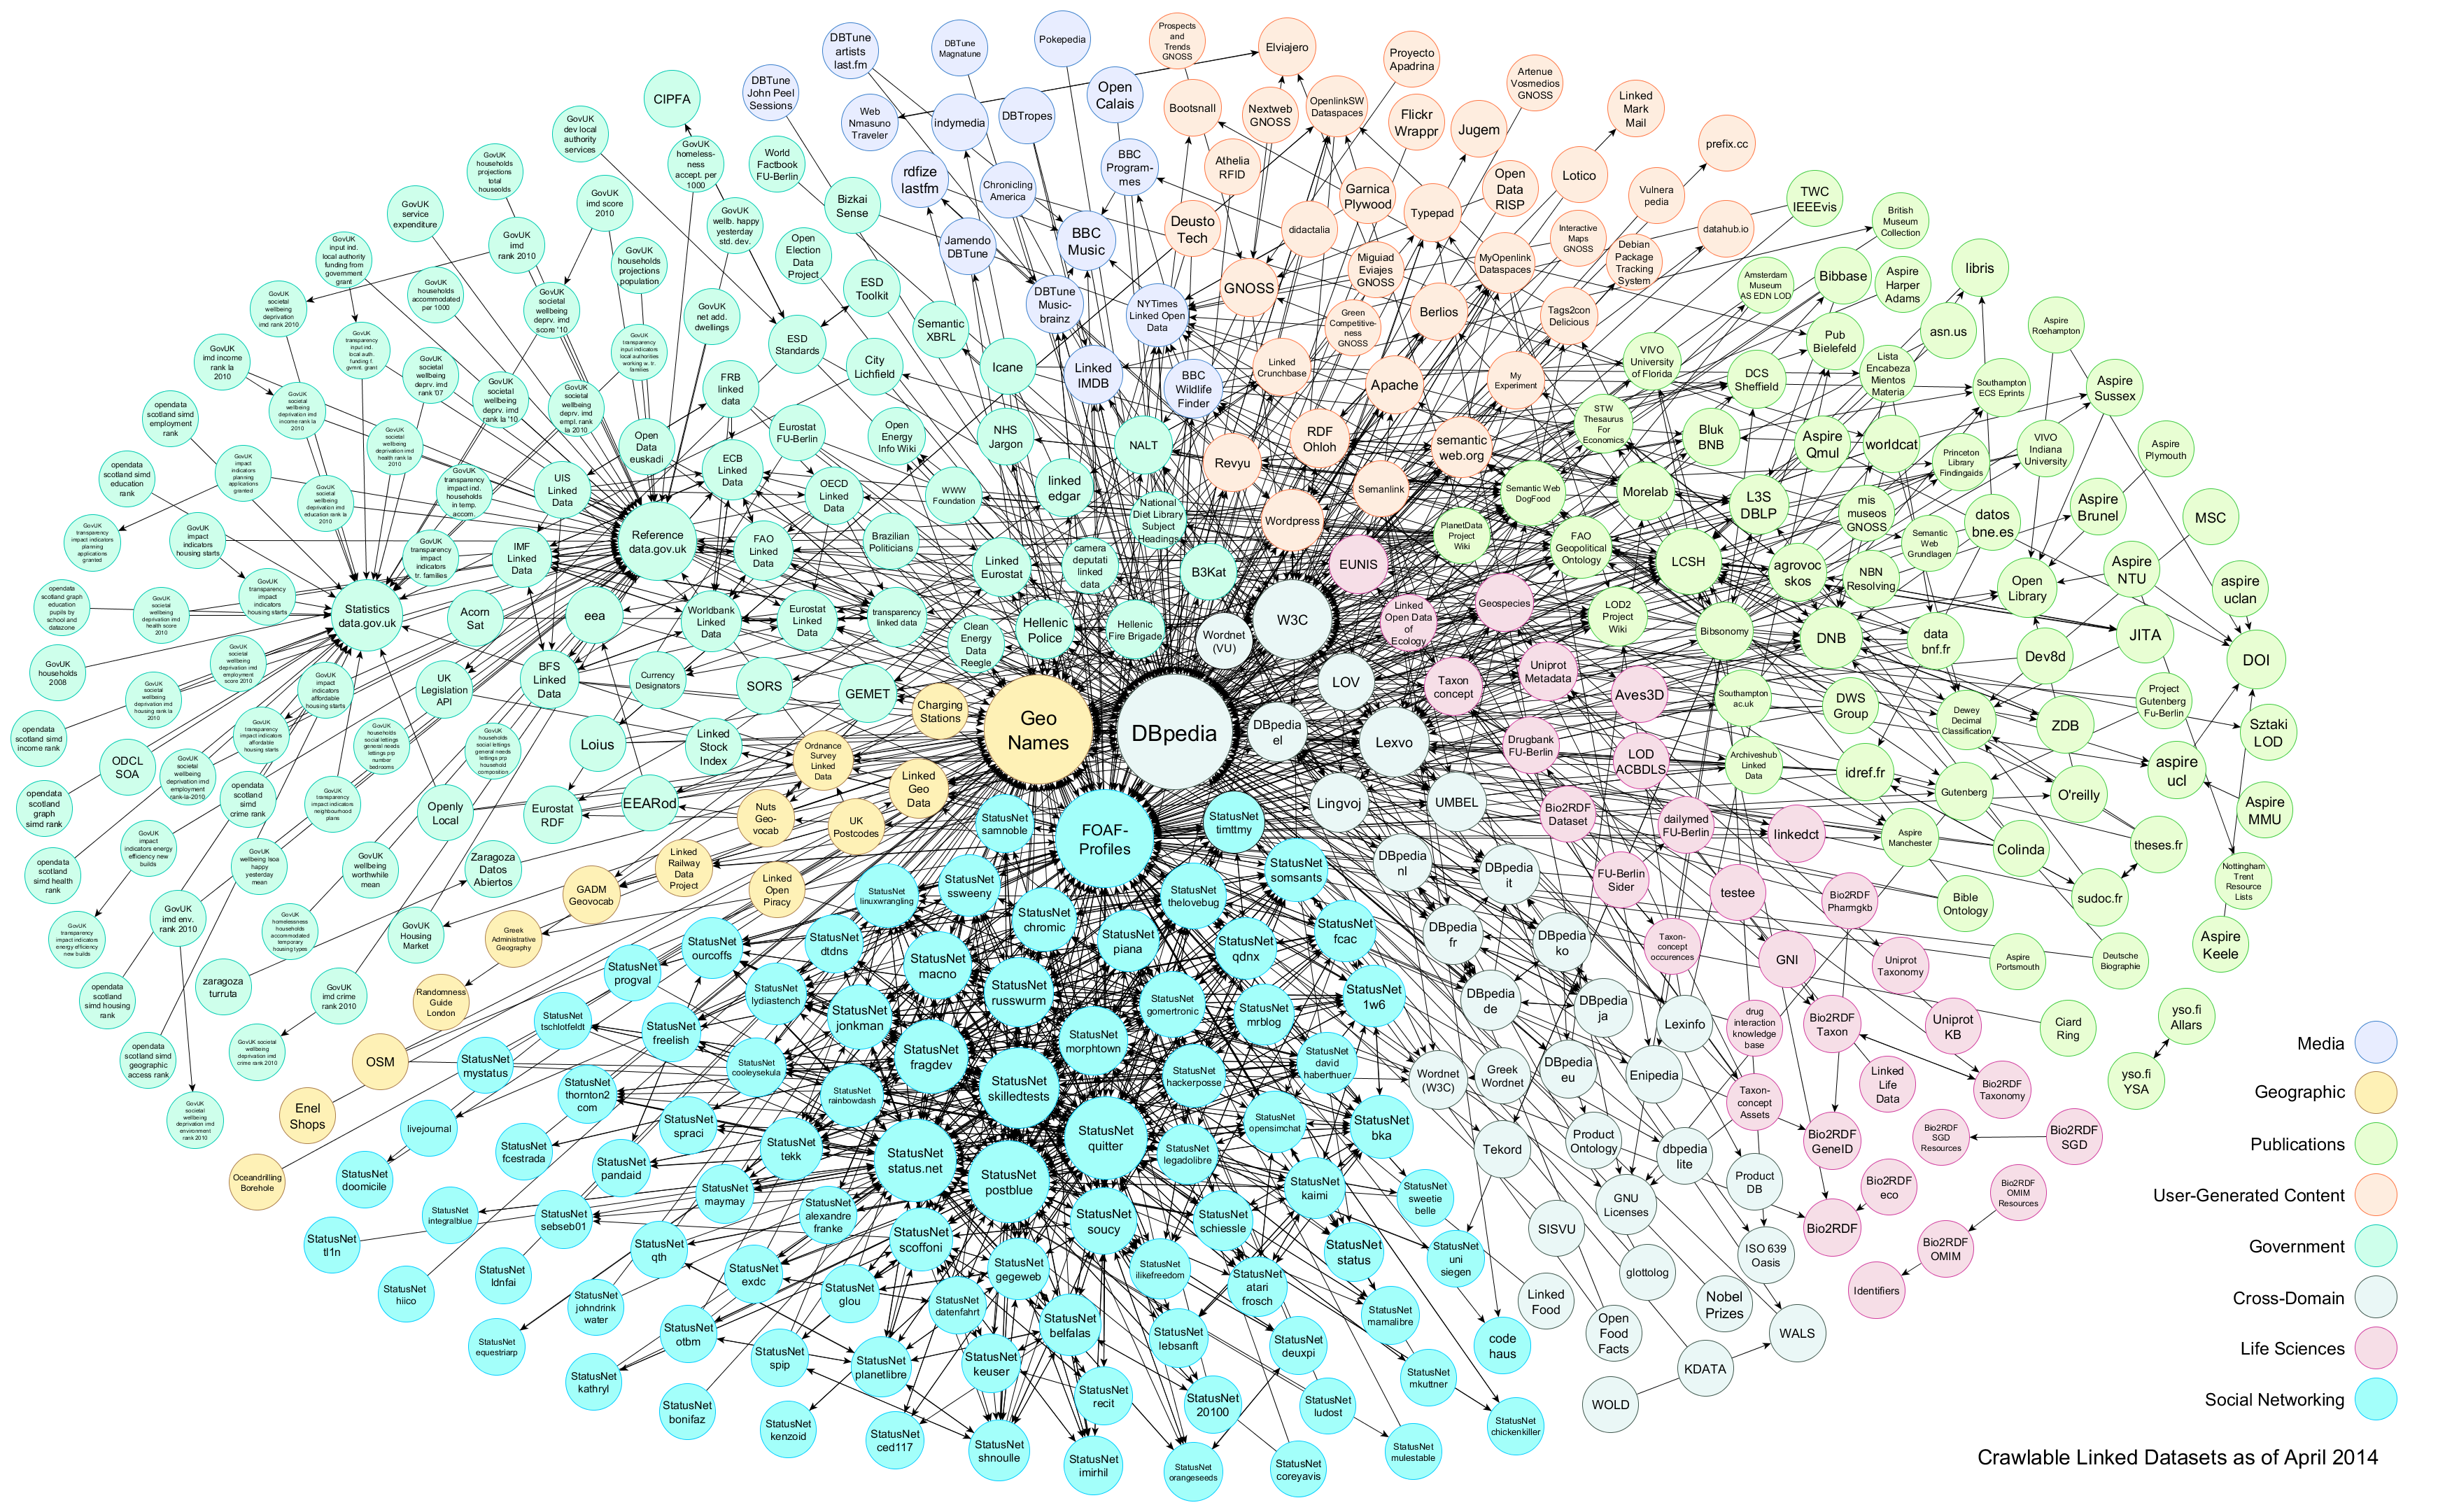
\includegraphics[width=8in]{lod2.png}  
%\end{sideways}
\caption{Linked Open Data cloud diagram.}
\label{fig:lod} 
\end{sidewaysfigure}

\subsubsection{RDF}
The Resource Description Framework (RDF) data model is used to describe resources with the subject, the predicate and the object triple, which can be viewed as ``a natural way to describe the vast majority of the data processed by machines''. 
By considering  RDF triples joined through shared URIs, one gets from a triple model to a graph data model\footnote{Resource Description Framework (RDF): Concepts and Abstract Syntax \url{https://www.w3.org/TR/2004/REC-rdf-concepts-20040210/#section-Concepts} (accessed Feb 2016)}, i.e., as show in Figure \ref{fig:rdfgraph}, each triple can be seen as a potentially distributed arc of an oriented labeled multi-graph. 

\begin{figure}%[htbp]
\centering
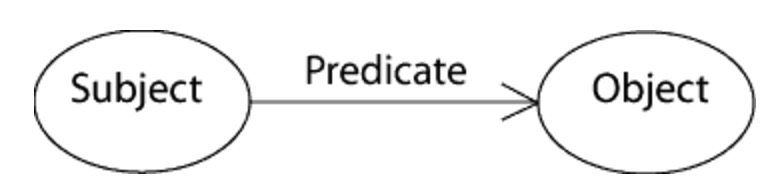
\includegraphics[width=5.3in]{rdfgraph.png}  
\caption{The triple as an arc in the graph data model of RDF.}
\label{fig:rdfgraph} 
\end{figure}

The subject represents the described resource. The predicate represents the property used to describe the resource. The object represents the value of the property for the described resource. Any user can define and describe any resource with this model. 
For example, to formalize the fact that the user kingRauk is the owner of the question \footnote{\url{http://stackoverflow.com/questions/16772071/sort-dict-by-value-python} (accessed Feb 2016)} from the Q\&A site Stackoverflow, we can use a triple 
\begin{itemize}
\item which subject <\url{http://stackoverflow.com/users/1214235/kingrauk}> is the URI that identifies the user who created the question,
\item which predicate <\url{http://rdfs.org/sioc/ns#owner_of}> is the URI that identifies the ownership property,
\item which object <\url{http://stackoverflow.com/questions/16772071/sort-dict-by-value-python}> is the URI that identifies the question.
\end{itemize}

Similarly, we can create another triple to formalize the fact that an answer is a reply to a question post:

\begin{itemize}
\item{its subject <\url{http://stackoverflow.com/questions/16772071/sort-dict-by-value-python/16772088#16772088}> is the URI that identifies the answer to the question,}
\item{its predicate <\url{http://rdfs.org/sioc/ns#reply_of}> is the URI that identifies the property \textit{reply of},}
\item{its object <\url{http://stackoverflow.com/questions/16772071/sort-dict-by-value-python}> is the URI that identifies the replied question.}
\end{itemize}
Alternatively, we can also create another triple to formalize the same fact where we can find the predicate 'reply\_of' is the inverse relation of 'has\_reply'. With respectively:
\begin{itemize}
\item{its subject <\url{http://stackoverflow.com/questions/16772071/sort-dict-by-value-python}> is the URI that identifies the replied question,}
\item{its predicate <\url{http://rdfs.org/sioc/ns#has_reply}> is the URI that identifies the property \textit{has reply}, the inverse relation of \textit{reply of},}
\item{its object <\url{http://stackoverflow.com/questions/16772071/sort-dict-by-value-python/16772088#16772088}> is the URI that identifies the answer to the question.}
\end{itemize}


\subsubsection{RDFS and OWL}
An ontology is ``a set of representational primitives with which to model a domain of knowledge or discourse. The representational primitives are typically classes (or sets), attributes (or properties), and relationships (or relations among class members). The definitions of the representational primitives include information about their meaning and constraints on their logically consistent application''~\cite{liu2009encyclopedia}.

RDF enables people to describe resources and RDF Schema (RDFS) provides the basic primitives to define properties and classes. From the definition given by the W3C\footnote{\url{https://www.w3.org/TR/rdf-schema/} (accessed Feb 2016)}, RDFS is a language to define RDF vocabularies in order to represent RDF data. RDFS primitives extend the basic RDF vocabulary; they mainly enable to declare classes, properties, hierarchies of classes and hierarchies of properties, and to associate labels and comments in Natural Language to classes and properties. 
The Web Ontology Language (OWL) builds on top of RDFS and provides a language for defining ontologies which enable richer integration and interoperability of data among descriptive communities. From the definition given by the W3C\footnote{\url{https://www.w3.org/OWL/} (accessed Feb 2016)}, OWL is a Semantic Web language designed to represent rich and complex knowledge about things, groups of things, and relations between things. While RDFS primitives enable to \textit{declare} atomic classes and properties, OWL primitives enables to  \textit{define} classes and properties. 
%NOTE Cath add a description of SKOS only if needed.

%NOTE FAB: then you should have a section on the vocabularies uou reuse with SIOC but also Dublin Core and FOAF no ? SKOS? when I look at section " QASM Vocabulary: formalize latent information" I think you use and could use more vocabularies than SIOC and they should all be introduced here.

\subsubsection{Vocabularies used in this thesis}
In this thesis we needed to represent users, posted questions and answers, communities, topics. Thus it is necessary to define an ontology for specific domain knowledge. We list the related and popular vocabularies used in our work.


\textbf{SIOC}\footnote{\url{https://www.w3.org/Submission/sioc-spec/} (accessed Feb 2016)} refers to the \textit{Semantically-Interlinked Online Communities} ontology, which provides the main concepts and properties to describe online communitiy sites, such as weblogs, forums, message boards, wikis. These websites contain huge amounts of valuable information and the SIOC ontology tries to solve the problem that online community sites are like islands without bridges connecting them. It uses semantic Web technologies to describe both the structure and content information in these online communities. It also allows us to link these information to related online communities. Fig \ref{fig:siocontos} shows an overview of the SIOC ontology. It mainly formalizes community users and related activities in online communities.
 
\begin{figure}%[htbp]
\centering
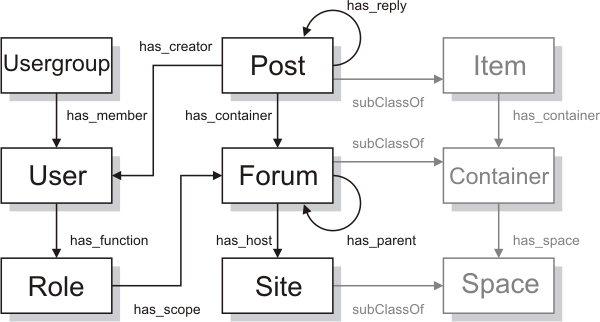
\includegraphics[width=5.3in]{sioconto.png}  
\caption{Overview of the SIOC ontology.}
\label{fig:siocontos} 
\end{figure}

The SIOC ``user' primitive extends the \textbf{FOAF}\footnote{\url{http://xmlns.com/foaf/spec/} (accessed Feb 2016)} ontology, which is another popular ontology to describe people and relationships between people. FOAF is a project devoted to linking people and information using the Web. SIOC ontology mainly extends FOAF Core'. It describes characteristics of people and social groups that are independent of time and technology. It includes classes such as OnlineAccount', 'OnlineGamingAccount' 'Organization', and 'Person'. Compared with SIOC, FOAF is not focusing on online communities and the user-generated content aspects. 
 
\textbf{Dublin Core}\footnote{\url{http://dublincore.org/documents/dcmi-terms/} (accessed Feb 2016)} specification provides term definitions that focus on issues of resource discovery, document description and related concepts useful for cultural heritage and digital library applications. It is used to describe Web resources, such as Web pages, images, videos, but also physical resources such as CD, books. Dublin Core Metadata may be used for multiple purposes, from simple resource description, to combining metadata vocabularies of different metadata standards, to providing interoperability for metadata vocabularies in the Linked Data cloud and Semantic Web implementations. It is also not specific for online communities and user-generated content.

\textbf{SKOS}\footnote{\url{https://www.w3.org/2004/02/skos/intro} (accessed Feb 2016)} stands for Simple Knowledge Organization Systems. It is a standard recommended by the W3C to formalize thesauri, classification schemes, subject heading systems and taxonomies within the framework of the Semantic Web. It enables to formalize the semantic relations between resources, such as 'narrower', 'boarder' and related'. It also enable to describe concepts and labels which are often used in online communities. 
In our work on formalizing the latent information, which is beneath the data, we can reuse SKOS primitives to formalize a topic. Moreover, our work shows use cases inviting to extend SKOS with new primitives enabling to formalize to what extent a user is interested in a topic.

 
\section{Context of the OCKTOPUS project: find the value of user-generated content}
Over the past 15 years, along with the success of the Social Web, online communities have progressively produced massive amounts of user-generated content collaboratively.
While some of these communities are highly structured and produce high-quality content (e.g., open-source software, Wikipedia), the level of discussions found within less structured forums remains highly variable. Coupled with their explosive growth, the lower quality of structure in online open forums makes it hard to retrieve relevant and valuable answers to users' search queries, and subsequently diminishes the social and economic value of this content.

The objective of the OCKTOPUS project\footnote{\url{https://alcmeon.com/ocktopus/} (accessed Feb 2016)} is to increase the potential social and economic benefit of this user-generated content, by transforming it into useful knowledge which can be shared and reused broadly. 
One of the targeted and easily-understandable output of the project is a demonstration platform which can be used to input a newly-formulated question, search online forums for a similar already-answered question, and display a unique user-generated answer associated with these similar questions.
This demonstration platform is built around the idea that finding relevant high-quality answers can be broken down in two steps:
\begin{itemize}
\item{Triage user-generated content to extract gold (knowledge structured as pairs of questions and answers) from ore (random discussions)}
\item{Given a newly-formulated question, retrieve relevant similar questions within the gold.}
\end{itemize}
OCKTOPUS therefore investigates newer data mining techniques based on the proper assessment 1) of the organizational traits of online communities, 2) of the tree-structure of online discussions, and 3) of the temporal dynamics of large typed semantic user-user graphs to help improve the automatic classification and triage the unstructured online content.



\section{Overlapping Community Detection}
We distinguish between three kinds of approaches for community detection, depending on their characteristics: Graph-based methods relying on the network structure; Clustering methods based on the similarity of user profiles; Probabilistic graphical models based on network structure and/or user profiles.

\subsection{Graph-based Methods}
A first and direct solution for detecting communities from UGC data is to extract an implicit network structure (such as a question-answer network, a co-answer network, etc.) from interaction traces to come down to a traditional community detection problem on social networks. Since intuitively, users are grouped by interests, and most of their interactions are based on shared interests, it is reasonable to induce a network structure from these interactions and then run community detection algorithms on the network. Many classical algorithms have been developed such as~\cite{DBLP:journals/csur/XieKS13}\cite{ahn2010link}. There are many constraints when adopting these methods. First, they do not take into account node attributes nor link attributes. Take co-answer network as an example, where nodes represent users and links represent users answering the same questions. In case two users are connected, these methods can only indicate that they have answered the same questions many times. They cannot provide the information whether they have answered questions on the same topic or on different topics. Second, some of the works adopting this approach cannot detect overlapping communities, while other works such as~\cite{DBLP:journals/csur/XieKS13} address this problem.

\subsection{Clustering Methods}
Community detection can also be envisioned as a clustering problem. By computing similarities between user profiles, one can detect communities according to clustering results. The choice of the similarity metrics is quite important and influences clustering results. 
To find similar interests, we first have to define the distance between user's interests and the definition of this distance has a strong influence on the clustering results. For instance, we can consider a bag of weighted tags to represent an interest, then compute the weighted tag distance to define the interest distance between two users.
Clustering methods, such as~\cite{DBLP:conf/sigmod/XuKWCC12}\cite{DBLP:conf/icwsm/GargiLMY11}, group users according to their features. They do not take the network structure into consideration. Moreover, some clustering algorithms normally output hard-partition communities i.e. one user can only be assigned to one community. However, in the scenario we are interested in, a user often has more than one interest and should be assigned to more than one group simultaneously. This is a constraint for those hard-partition algorithms. 
\cite{Chang:2013} use spectral clustering to detect topics from the graph of tag co-occurrence. Compared to it, our approach is more efficient since we only run spectral clustering on a co-occurrence graph of selected tags (only 10\% of all the tags). Besides, \cite{Chang:2013} does not give any details on how to compute the topic tag distribution and user topic distribution, while we do.

\subsection{Probabilistic Graphical Models}
A third approach consists in using a probabilistic graphical model for both the user profiles and the network structure to solve community detection problem. For example, \cite{DBLP:conf/isi/ZhangQGFY07} transform links to binary node attributes, then use a Latent Dirichlet allocation (LDA) model to detect communities. \cite{journals/jasis/SunL13} use a LDA-based method on social tagging systems where users label resources with tags, but they do not consider the problem of overlapping community detection.  \cite{tang2008arnetminer} use an extended LDA-based model to analyze academic social networks in order to find expert authors, papers and conferences. A problem of these LDA-based models is that they normally assume soft-membership~\cite{yang2013community} which means that a user cannot have high probabilities to belong to several communities simultaneously. That is to say, the more communities a user belongs to, the less it belongs to each community (simply because probabilities have to sum to one). 
Moreover, \cite{mcdaid2010detecting} and \cite{lancichinetti2011finding} also use a statistic model to detect overlapping communities. The difference is that LDA-based models normally integrate topic detection which can be used to interpret detected communities while the two above cited methods only detect overlapping communities without any topic information on each detected communities.

\subsection{Discussion on community detection alternatives}
Table \ref{tab:methodcomparison} summarizes the main features of the three approaches. 
The columns 'nodes' and 'links' indicate whether each method uses this information.  
The column 'overlap' indicates whether a user can belong to different communities i.e. if the approach detects overlapping communities.  
The column 'membership' indicates if the method provides a measure of "how much one user belongs to one community". 
The column 'topic' indicates if the method generates a bag of words to represent a topic, which can be used to explain the main aspects of contents generated by the users in the community.

%TODO Fab: if there are differences between the methods you referenced in the three kinds of approaches you should add a line per reference in the table to show these differences.
%DONE in the summary section, I did this compartion between references. Here is just a summarizing of methods.

Graph-based approaches normally use link information while ignoring node attributes. Some of them cannot detect overlapping communities or provide membership ratios which are weights denoting to what extent a user belongs to a community. Most of these methods cannot identify the topic in each detected community. Clustering approaches use node attributes to group similar users. Some of their results are hard-partition communities, with no overlapping and no membership information. LDA-based models overcome the shortcomings of graph-based and clustering approaches, using both node attributes and link information. Besides, LDA-based models normally combine community detection with topic detection, which could be used to interpret detected communities. Our proposed method is similar to LDA-based methods, in that it also enables to detect overlapping communities and identify the topics at the same time. It differs from LDA-based methods in that it enables to consider a user having high probabilities to belong to several communities simultaneously while these methods normally assume soft-membership \cite{yang2013community}. In addition, our proposed method is much simpler and faster than LDA-based methods while preserving the quality of the detection.
For more details about community detection algorithms in graphs, we refer the readers to \cite{fortunato2010community} and \cite{DBLP:journals/csur/XieKS13}.
\begin{table}[htp]
\caption{Comparison of the main approaches and our method}
\label{tab:methodcomparison}
\centering
%\begin{tabular}{|p{28pt}|p{18pt}|p{18pt}|p{18pt}|p{25pt}|p{16pt}|}
\begin{tabular}{|c|c|c|c|c|c|}
\hline
 &nodes &links & overlap & membership & topic\\
\hline
Graph-based methods & no & yes & few & few &no\\
\hline
Clustering methods & yes & no & few & few &no\\
\hline
Probabilistic graphical model& yes & yes & yes & yes &yes\\
\hline
%\hline
\end{tabular}
\end{table}



\section{Topic Modeling: Uncover the Hidden Thematic Structure}

According to David M. Blei\footnote{\url{https://www.cs.princeton.edu/~blei/topicmodeling.html} (accessed Feb 2016)}, "Topic models are a suite of algorithms that uncover the hidden thematic structure in document collections. These algorithms help us develop new ways to search, browse and summarize large archives of texts." For example, "guitar" and "music" will appear more often in documents about music, "law" and "lawsuit" will appear more often in documents about laws, and "the" and "is" will appear equally in both documents. A document normally contains multiple different topics in different proportions. For example, a document on music copyright lawsuit, could be 30\% about music and 70\% about laws.

Latent Semantic Analysis (LSA or LSI)~\cite{chp2deerwester1990indexing} \cite{chp2landauer1997solution} is an early topic model based on the factorization of document-word occurrence matrix. By using singular value decomposition (SVD), it can find a linear combination of topics for each document.
Probabilistic Latent Semantic Analysis (PLSA), also known as Probabilistic Latent Semantic Indexing (PLSI)~\cite{chp2papadimitriou1998latent}\cite{chp2hofmann1999probabilistic} is a generative statistic model to estimate a low-dimensional representation of the observed variables. Latent Dirichlet Allocation (LDA)~\cite{blei2003latent} is also a generative statistic model that uses observed variables to explain unobserved latent variables, which is a generalization of PLSI model. \cite{griffiths2004finding} \cite{chp2griffiths2002probabilistic} use Gibbs sampling to infer the latent variables in LDA model and introduce some applications of LDA model. Many other topic models are extensions of the LDA model. For example, Hierarchical Latent Dirichlet Allocation (HLDA)~\cite{chp2DBLP:conf/nips/2003} is a topic model that finds a hierarchy of topics. The structure of the hierarchy is determined by the data. Dynamic topic models (DTM)~\cite{chp2blei2006dynamic} discover topics that change over time and how individual documents predict that change. Correlated Topic Models (CTM)~\cite{chp2blei2006correlated} discover correlation structures between topics, etc.

Topic modeling is an active field in text mining and machine learning and we refer the readers to \cite{chp2Blei:2012:PTM:2133806.2133826} for a high level view and summary of the topic modeling research area and also for several exciting future research directions. One of them deals with the development of evaluation methods, \textit{"How can we compare topic models based on how interpretable they are?"}.

Another interesting research problem related to topic modeling is \textit{how to automatically label the generated topics?} \cite{chp2cano2014automatictopiclabeling} \cite{chp2hulpus2013unsupervisedtopiclabeling} \cite{chp2aletras2014labelling} \cite{chp6OnConceptualLabelingOfBagOfWords} \cite{chp2lau2011automaticlabeling} 
Typically, users of topic modeling approaches have to interpret the results and manually generate labels for topics for further processing, classification, visualization or analysis. Therefore, in this context, "labelling" means the problem of finding one or more phrases, or concepts, which can sufficiently cover, represent or describe the topic. The problem then is defined as the automation of the topic labelling.



\section{Temporal Analysis: integrate temporal analysis within topic modeling}

There is an increasing research interest for the temporal modeling of online communities and several methods have been proposed. 

\cite{wang2006topics} introduced \textit{Topic Over Time} (TOT), which jointly models topics and timestamps by assuming that words and timestamps are both generated by latent topics. Therefore, the parameter estimation is able to discover topics that simultaneously capture word-word co-occurrences and word-timestamps co-occurrences. If some words co-occurre for a short period, their approach will create a topic with a narrow time distribution. If some words co-occurre across a long time, their approach will create a topic with broad time distribution. The novelty of TOT  is that it treats time as an observed continuous variable rather than a Markov process. Besides, the meaning of topics remains constant while the topic themselves change over time. 
\cite{chp2blei2006dynamic} proposed a dynamic topic model that treats the temporal dimension as a Markov process where the meaning of topics changes over time. \cite{chp2onlineldaalsumait2008line} also studied topic changes over time, but they focus on proposing an online method to extract topics from a stream of data.
\cite{chp2wang2007mining} address the problem of mining correlated busty topic patterns from coordinated text streams (e.g. the same news in different medias or in different languages). They proposed a mixture model which is an extension of PLSA~\cite{hofmann1999probabilistic} model to detect topic evolution from text streams by comparing topics in consecutive time intervals. 
\cite{chp2yao2010detecting} and \cite{chp2yao2012bursty} proposed a sliding window and graph partition based approach to detect burst event/topic in tags. 
\cite{chp7diao2012finding} proposed a TimeUserLDA model to find bursty topic from microblogs. It considers both user personal topic trends and global topic trends and detect bursty topics from the extracted topics over time distribution.
\cite{yin2013unified}  proposed a PLSA-based~\cite{hofmann1999probabilistic} model to separate temporary topics from stable topics. Temporal topics are on popular real-life events, e.g. breaking news. It will lead to a burst in online community discussions with a large amount of user-generated content in a short time period. Stable topics are often users' regular interests and daily routine discussions which always exist and do not evolve a lot in a long time period. \cite{hu2014user} jointly model latent user groups and temporal topics to detect group-level temporal topics.

Compared with these works, our model not only captures topics and expertise, it  can also detect topic dynamics both at the global community level and at the individual user level. Besides, we propose a post-process method to extract both topic-time and time-topic distribution. The time-over-topic distribution are usually ignored.



\section{Q\&A Sites Management}
%NOTE Cath this title is not correct: these are not the research question you want to address (these are not the one listed at the end of the chapter). These are rather use cases or scenarios you want to answer, or for which you want to provide usefull material. Or maybe this is your state of the art on Q\&A site management? This should be explained in the introduction of this section
%NOTE Zide yes, these should be tasks rather than research questions. In order to solve these tasks, we expand the research.
%Note2 Cath -> then at least make it clear in the introduction of this section
\subsection{Expert Detection: find the "core" user}
Research related on expert identification in Q\&A sites is mainly based on link analysis and topic modeling techniques. The general purpose of expert detection is normally to support the question routing task which essentially consists in finding the most relevant experts to answer a newly submitted question. 

\cite{zhang2007expertise} is not specific to Q\&A community and focuses on a broader website category: help-seeking websites. It tested pagerank and hits algorithms to detect expert in such websites. Pagerank and Hit are well known authority algorithms in directed graph analysis. By constructing a directed graph of the users'network, they could apply these algorithms to find the most important node in the graph according to these centrality metrics. Besides, they proposed the Z-score measure to evaluate expertise. Compared with simple statistic measures, for instance the number of best answers provided by a user, the Z-score measure uses both the number of questions and the number of answers posted by a user. Similarly, \cite{jurczyk2007discovering} use the HITS algorithm to discover authorities users. \cite{li2010routing} propose a probability model to estimate users' expertise for question routing task. 

\cite{chp2Zhou:2012:TPM:2396761.2398493} address a core problem in applying the previous techniques to Q\&A site. They argue that most of the previous works in expert finding are based on link analysis while ignoring the topical similarity among users and user expertise and user reputation. They proposed a topic-sensitive probabilistic model to find experts in Q\&A sites. This model is based on LDA. Then they generate a topic-similar graph based on the result of topic model. Finally a PageRank algorithm is applied to find the experts. They compared their work with many state of the art link analysis algorithms and showed a gain in the experiment.

\cite{chp2Pal:2010:Expert:evolution} on the other side proposed a temporal pattern based expert detecting method. The temporal pattern is based on the reputation system of Q\&A sites where a user having a high reputation is considered as an expert. Their approach uses a supervised learning algorithm to distinguish experts from normal users. The limitation of this work is that it cannot find in which topics people are specialized.

\cite{chp2Bouguessa:2008:Identify:authority:indegree} proposed a method using link analysis techniques to find a list of expert users based on the in-degree of authority, which is computed based on the number of best answers provided by a user. Then they use the Bayesian Information Criterion (BIC) to estimate the authority score of a user. Therefore, experts are chosen according to their authority score. Their expertiment was done on Yahoo Answers.


Rather than detecting global experts, another kind of works uses topic models to detect topic level experts. \cite{guo2008tapping} proposed a generative model by leveraging the category information of questions on certain Q\&A sites. \cite{yang2013cqarank} jointly model topics and expertise by  integrating a Gaussian Mixture Model to capture vote information. \cite{Chang:2013} propose a spectral clustering based topic model. 
\cite{ma2015tri} propose a generative model to model the triple role of users (as askers, answerers, and voters). Our contribution extends this line of work. 

There are also approaches applying machine learning techniques to perform expert detection. \cite{ji2013learning} combine topic models outputs and statistic features and apply a pair-wised learning to obtain a ranked model and recommend expert users for a question. \cite{pal2011early} apply machine learning algorithms to identify experts from their early behavior. \cite{anderson2012discovering} perform an in-depth study of StackOverflow and show that expert users tend to answer questions more quickly and gain high reputation by higher activity. Their work is based on features extraction and machine learning algorithms to predict whether a question has a long-term value and whether a question has been sufficiently answered. Their results show that votes information can indicate a user's expertise level while currently, this kind of work normally relies on the outputs of topic models.

\subsection{Question Routing: recommend new questions to users}

\cite{Guo:2008:TPQ:1458082.1458204} %UQA
try to solve question routing problem, which we categorized as Q5. They proposed an LDA-like probability model to find the latent topic of users and latent topic of questions and answers. Then based on this topic information, they can route a new question to a user which has the same topic distribution.
\cite{yang2013cqarank} %TEM
proposed a Topic Expertise Model which is also an LDA-like probability model but combined with a Gauss Mixture Model (GMM) model to detect experts in Q\&A sites. The probability model is mainly used for extracting topics from tags and words in Q\&A and it contains two LDA processes: 'user-topic-tag' and 'user-topic-content'. The GMM is used for analyzing users expertise on each topics. The output includes topic-tag distribution, user-topic distribution, topic-word distribution and the users' topic-expertise matrix. Then according to these outputs, they can identify the top tags of a topic, top users of a topic and top experts of a topic. The experiments show they can outperform the state-of-the-art probability model in Q\&A sites.


\cite{Chang:2013}
proposed a recommendation model, which integrates topical expertise and availability of users, to recommend reactive answerers and commenters for a question. It constructs a similarity matrix between tags, and runs spectral clustering algorithm over it. Then a cluster of tags can be viewed as a topic. But unlike LDA, spectral clustering can not output the topic-tag distribution which will limit the flexibility of afterwards application. The paper proposed a question-topic distribution, but it dose not mention how to compute it. So the conclusion that spectral clustering can out perform LDA is not clear. And spectral clustering is hard partition of tags, while LDA can give proportion that a tag belong to a topic. 



\subsection{Similar Question: find questions which have been answered}

\cite{anderson2012discovering} investigate the general characteristics of the StackOverflow dataset. A contribution of this work is to predict the long-term value of a question. They find strong evidences that only 37\% of favorites for a question arrive within the time frame when the question is being answered. Actually the content in Q\&A sites mainly serves two kinds of people: the people who ask questions and the people who search through previous questions. So, if a question has a long-term value, it is more likely to be searched for again. Finding out these questions could improve the result of searching for similar questions. 
They developed four categories of features for learning. They include: 4 questioner features which are related to questioner's behaviors; 8 activity and Q/A quality measures which are extracted from questions and answers; 8 community process features which are related the reputation of answers; and 7 temporal process features which are generated from the time information of the Q/A activity.
Then they treat this problem as a binary classification task and use a machine learning technique to predict whether a question has a long-term value. They compare their work with a baseline which only uses upvote and downvote features. 

\cite{chp2jeon2005finding}
discuss methods for question retrieval that are based on using the similarity between answers. It proposed a translation-based retrieval model to find similar questions. The experiment shows that it is possible to find semantically similar questions with relatively few overlapping words.
They found that question titles can provide the best performance for retrieving similar question. This work is based on the intuition that most of the people do not check whether their question has been already asked which leads to a situation where there can be many semantically identical questions. Therefore, they use the similarity between answers to group similar questions. A translation model based algorithm is proposed to calculate the similarity between answers. For example, this model can provide a similarity score between 'bmp' and 'jpg'. Experiments show that the model can outperform other language models and similarity metrics. 

%subsubsection{Probabilistic Question Recommendation for Question Answering Communities}
\cite{chp2Qu:2009:WWW:PLSA:SimlarQ} 
present a probabilistic latent semantic analysis (PLSA) approach to compute the probability that a user will answer a question. 
They actually build a user-interest-question model. PLSA and LDA are quite similar and both are topic models, and LDA could be viewed as an extension of PLSA. The experiment shows that topic features based similarity can outperform cosine distance based similarity. \cite{chp2Wu:2008:PLSA:SimlarQ} also used PLSA to recommend questions.

Table \ref{tab:workcompare} provides a comparison of the above described works.

%NOTE FAB: I changed the following table to a "sidewaystable" without tiny you should do that for any large table
%d'accord
\begin{sidewaystable}%[!hbp]
%\tiny
\centering
\begin{tabular}{|c|c|c|c|c|c|c|}
\hline
&Expert & Routing &SimilarQ& Method & Dataset &Topic   \\
\hline
\cite{chp2jeon2005finding} 2005&no&no&yes&Probability Model&Naver\footnote{A leading Q\&A sites in South Korea} & no \\
\hline
 \cite{zhang2007expertise} 2007& yes &no& no& PageRank,Hits&Forum&no  \\
\hline
\cite{Guo:2008:TPQ:1458082.1458204} 2008 & no&yes&no&LDA based&StackOverflow&yes\\
\hline
\cite{chp2Qu:2009:WWW:PLSA:SimlarQ} 2008,\cite{chp2Wu:2008:PLSA:SimlarQ}2008  & no&yes&yes&PLSA&Yahoo,Wenda & yes \\
\hline
\cite{chp2Bouguessa:2008:Identify:authority:indegree} 2008 & yes&no&no&Link Analysis&Yahoo&no\\
\hline
\cite{chp2Pal:2010:Expert:evolution} 2010&yes&no&no&Supervise Learning&StackOverflow&no \\
\hline
\cite{anderson2012discovering} 2012& no&no&yes&Supervise Learning&StackOverflow&no \\
\hline
\cite{chp2Zhou:2012:TPM:2396761.2398493} 2012 & yes & no & no&LDA based &StackOverflow&yes\\
\hline
\cite{yang2013cqarank} 2013& yes&yes&yes& LDA based&StackOverflow&yes   \\
\hline
\cite{Chang:2013}2013 & yes&yes&no& SpectralClustering&StackOverflow&yes  \\
\hline
\end{tabular}
\caption{Comparison of several works in Q\&A sites. 'Expert' denotes 'Expert detection', 'Routing' denotes 'Question Routing', 'Similar' denotes 'Similar Question Finding', 'Method' denotes 'Proposed algorithm', 'Dataset' denotes 'Experiment Data', and 'Topic' denotes 'Topic Detection'}
\label{tab:workcompare}
\end{sidewaystable}



\section{Research Questions: the focus of this thesis}
In this section we summerize the research questions we will address in this thesis and we position our contribution for each of them. 

\subsection{How to formalize user-generated content?}
    
    \begin{table}[htp]
        \centering
        \begin{tabular}{c c c c c}
        &
        \begin{turn}{270}
            \cite{chp2socialsemanticminingDBLP:series/synthesis/2015Omitola} \end{turn} 
        &
        \begin{turn}{270} 
            \cite{chp2siocontoDBLP:conf/atal/PassantBBD09}
        \end{turn}
        &
        \begin{turn}{270} 
            \cite{chp2usermodelingplumbaum2015user}
        \end{turn}
        &
        \begin{turn}{270}
        our work
        \end{turn}
        \\ \hline
        Social media mining & yes & yes & no & yes \\ \hline
        User Behaviour modeling & yes & yes & yes &yes \\ \hline
        User interesting modeling & no &yes & no & yes\\ \hline
        User activity modeling & no & no & no & yes\\ \hline
        User expertise modeling & no & no & no & yes \\ \hline
        Topic based modeling & yes & no & no &yes \\ \hline
        \end{tabular}
        \caption{Position of our work regarding to the first research question}
        \label{tab:rq1compare}
    \end{table}
Compared to state of the art approaches, we use social media mining techniques to extract topical dynamic, topical activity, topics and topical expertise from user-generated content. Then we integrate these extracted information into the original dataset in order to provide more functionality for further use. We will detail this work in Chapter \ref{chap:qasm}. 
    


\subsection{How can we identify the common topics binding users together?}
    
    \begin{table}[htp]
        \centering
        \begin{tabular}{c c c c c c}
        &
        \begin{turn}{270}
            \cite{blei2003latent} \end{turn} 
        &
        \begin{turn}{270} 
            \cite{Chang:2013} 
        \end{turn}
        &
        \begin{turn}{270} 
            \cite{yang2013cqarank}
        \end{turn}
        &
        \begin{turn}{270}
            \cite{hu2014user}
        \end{turn}
        &
        \begin{turn}{270}
        our work
        \end{turn}
        \\ \hline
        Model & PGM & SC & PGM & PGM & SC\\ \hline
        Simplicity & no & yes & no & no & yes\\ \hline
        Sub-topic & no & no & no & no &  yes \\ \hline
        Iterations & yes & no & yes& yes & no \\ \hline
        
        \end{tabular}
        \caption{Position of our work regarding to the first research question, \textit{PGM}: Probabilistic Graphical Model, \textit{SC}: Spectral Clustering}
        \label{tab:rq2compare}
    \end{table}
Compared to the state of the art approaches, we focus on the simplicity and efficient aspect of the proposed method. Based on a prefix-tree structure, our method can also extract sub topics from a topic. We detail this work in Chapter \ref{chap:ttd}.
    
    
    
\subsection{How can we generate a semantic label for topics?}



   \begin{table}[htp]
        \centering
        \begin{tabular}{c c c c c c}
        &
        \begin{turn}{270}
            \cite{chp6OnConceptualLabelingOfBagOfWords} 
        \end{turn} 
        &
        \begin{turn}{270} 
            \cite{chp2hulpus2013unsupervisedtopiclabeling} 
        \end{turn}
        &
        \begin{turn}{270} 
            \cite{chp2cano2014automatictopiclabeling}
        \end{turn}
        &
        \begin{turn}{270}
            \cite{chp2aletras2014labelling}
        \end{turn}
        &
        \begin{turn}{270}
        our work
        \end{turn}
        \\ \hline
        Extra information& Probase\footnote{\url{http://research.microsoft.com/en-us/projects/probase/} (accessed Feb 2016)} & DBpedia & no  & Bing\footnote{\url{https://www.bing.com/} (accessed Feb 2016)} results & DBpedia \\ \hline
        Method & MDL & DR Graph &S& Words Graph & DR Graph   \\ \hline
        User Study & no & yes & no & no&  yes \\ \hline
        Label Type & word & DR & word & words & DR \\ \hline
        
        \end{tabular}
        \caption{Position of our work regarding to the third research question, \textit{MDL}: Minimum Description Length, \textit{DR}: DBpedia Resource, \textit{S}: Summarization Algorithm,  }
    
        \label{tab:rq3compare}
    \end{table}
Compared to the state of the art approaches, we focus on extending our topic extraction method and on using DBpedia resources to automatically generate labels for bags of words composing topics. We also compare several graph centrality metrics to generate labels. We describe this work in Chapter \ref{chap:label}.
    
    
\subsection{How can we detect topic-based overlapping communities?}

    \begin{table}[htp]
        \centering
        \begin{tabular}{c c c c c c c}
        &
        \begin{turn}{270}
            \cite{raghavan2007near} 
        \end{turn} 
        &
        \begin{turn}{270}
            \cite{DBLP:journals/csur/XieKS13} 
        \end{turn} 
        &
        \begin{turn}{270} 
            \cite{girvan2002community}
        \end{turn}
        &
        \begin{turn}{270} 
            \cite{yang2013community}
        \end{turn}
        &
        \begin{turn}{270}
            \cite{hu2014user}
        \end{turn}
        &
        
        \begin{turn}{270}
        our work
        \end{turn}
        \\ \hline
        Method &LPA & LPA & HC & PGM &PGM & SC\\ \hline
        Info  & Graph & Graph &Graph & Graph, Content & Graph, Content& Graph, Content\\ \hline
        Interpret& no & no & no & yes & yes & yes \\ \hline
        %explained by topic
        Overlapping & no & yes & no & yes & yes & yes \\ \hline
        Simplicty & yes & yes & yes & no & no & yes \\ \hline
        \end{tabular}
        \caption{Position of our work regarding to the first research question, \textit{LPA}: Label Propagation Algorithm \textit{PGM}: Probabilistic Graphical Model, \textit{HC}: Hierarchical Clustering \textit{SC}: Spectral Clustering}
        \label{tab:rq4compare}
    \end{table}
Compared to the state of the art approaches, we focus on extending topic extraction methods to effectively detect overlapping communities. We describe this work in Chapter \ref{chap:ttd}.



    
\subsection{How can we extract topics-based expertise and temporal dynamics?}
    
    
        \begin{table}[htp]
        \centering
        \begin{tabular}{c c c c c c c c}
        &
        \begin{turn}{270}
            \cite{yang2013cqarank} 
        \end{turn} 
         &
        \begin{turn}{270}
            \cite{Chang:2013}  %sc
        \end{turn} 
        &
        \begin{turn}{270} 
            \cite{guo2008tapping} %uqa
        \end{turn}
        &
        \begin{turn}{270} 
            \cite{blei2003latent} %lda
        \end{turn}
        &
        \begin{turn}{270}
            \cite{hu2014user} %grostot
        \end{turn}
        &
        \begin{turn}{270}
            \cite{chp7diao2012finding} %fb
        \end{turn}
        &
        \begin{turn}{270}
        our work
        \end{turn}
        \\ \hline
        Model & PGM &SC & PGM & PGM & PGM & PGM& PGM\\ \hline
        Topic Dynamic & no & no & no & no & GL & GL,UL & GL, UL \\ \hline
        Expertise & yes & yes& no & no & yes &no &yes   \\ \hline
        User Activity& no & non-topical & no & no &topical & topical & topical \\ \hline
        \end{tabular}
        \caption{Position of our work regarding to the first research question, \textit{PGM}: Probabilistic Graphical Model, \textit{SC}: Spectral Clustering, \textit{GL}: global level, \textit{UL}: user level}
        \label{tab:rq5compare}
    \end{table}
Compared to the state of the art approaches, we integrate topic dynamics, users' activity and topic based expertise extraction together to solve several tasks related to Q\&A site. We describe this work in Chapter~\ref{chap:ttea}.